% template for Phoebe
%
\documentclass{phoebe}

% ---------------------------------------------------------------------
% Place your own packages here 
% ---------------------------------------------------------------------

\usepackage{blindtext}

% ---------------------------------------------------------------------
% Place your own commands here 
% ---------------------------------------------------------------------


% ---------------------------------------------------------------------
% Define some variables
% ---------------------------------------------------------------------

\title[\LaTeX\ template \& style guide]{\phoebe\ -- Gazette Heidelberger Physik Studenten: \\\LaTeX\ template \& style guide} 
\author[F. Scheuermann \& C. Otte]{Fabian Scheuermann \and Christoph Otte}
\doi{10.1093/mnras/stac110}
\pubdate{2022.09.23}

 % load file with bibliography
\addbibresource{paper.bib}  

\defabstract{This is some text. \blindtext}

% ---------------------------------------------------------------------
% The main Document
% ---------------------------------------------------------------------


\begin{document}


% ---------------------------------------------------------------------
% Frontmatter
% ---------------------------------------------------------------------

\maketitle

% ---------------------------------------------------------------------
% Main Body of the article
% ---------------------------------------------------------------------


\section{ToDo}

Here is a list of things that need to be changed
\begin{itemize}
    \item Change the author and title macro to allow for a running title and running author (used in the header).
    \item Add affiliations to the authors?
    \item Center Abstract heading
    \item Footnote for corresponding author. 
\end{itemize}

here is a list of nice looking journals
\begin{itemize}
    \item \href{https://www.tatup.de/index.php/tatup/issue/view/173/180}{Zeitschrfit für Technikfolgenabschätzung in Theorie und Praxis (TATuP)}
\end{itemize}

\section{Introduction}

The quick brown fox jumps over the lazy dog

\Blindtext

\section{Examples}

\subsection{Math mode}

Here is a formula
\begin{equation}
    y = \int_0^\infty \frac{1}{x^2}\, \mathrm{d}x.
\end{equation}
They should always be punctuated. 

\subsection{Figures and Tables}

In Figure~\ref{fig:example} and Table~\ref{tab:example} we show an example for a figure and a table respectively. 
\begin{figure}
    \centering
    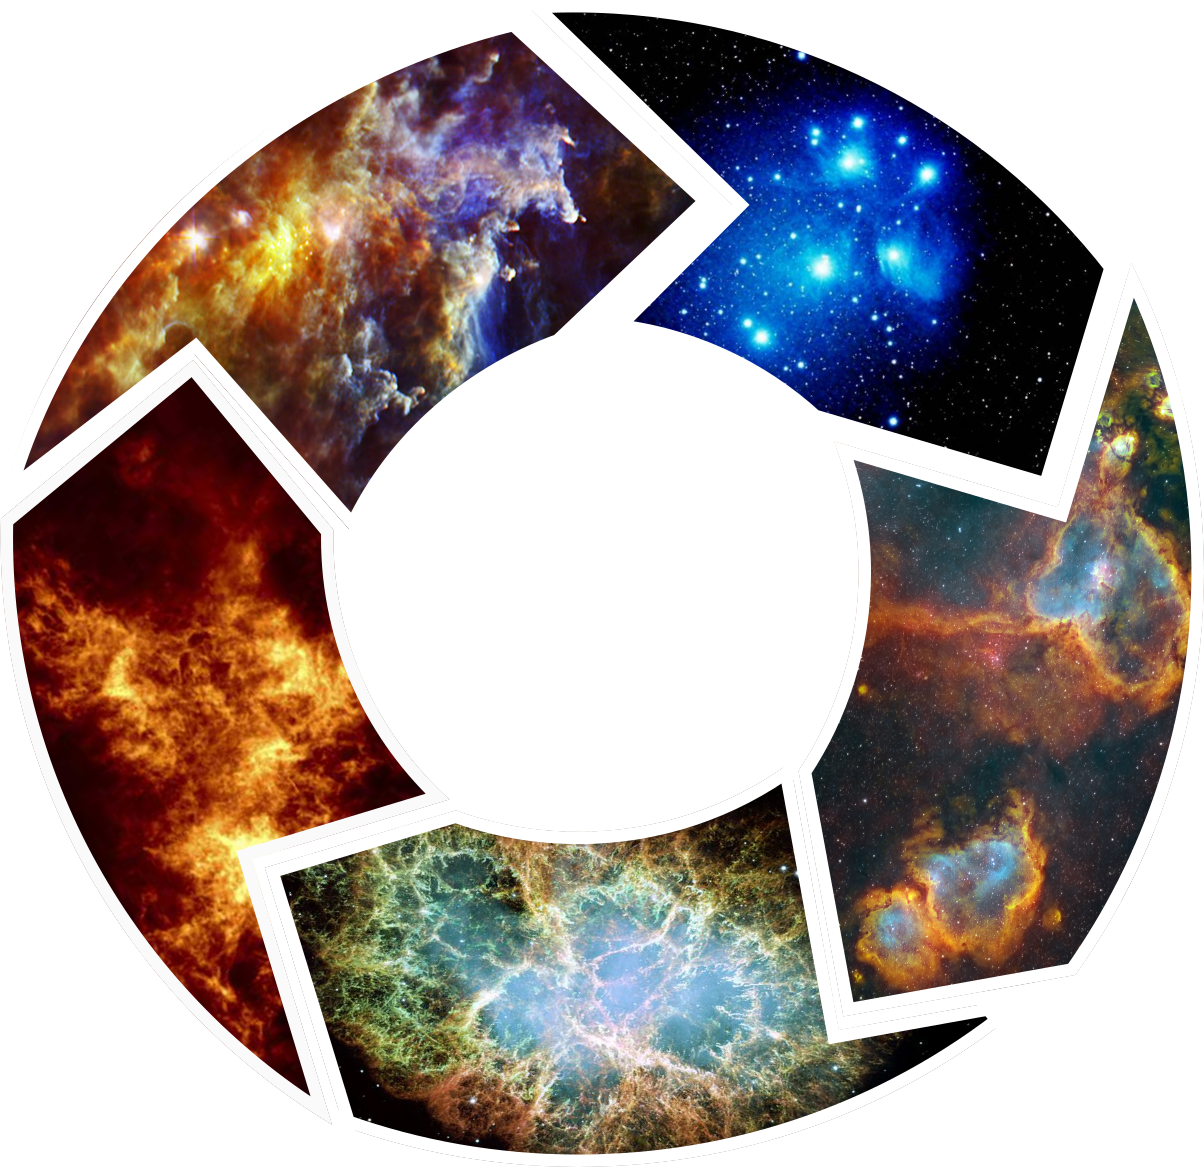
\includegraphics[width=0.8\columnwidth]{baryon_cycle}
    \caption{This is an example for a figure}
    \label{fig:example}
\end{figure}


\begin{table}
    \centering
    \caption{This is an example for a table}
    \begin{tabular}{cc}\toprule
        Column 1  & Column 2 \\\midrule
        1 & A \\
        2 & B \\
        3 & C \\\bottomrule
    \end{tabular}
    \label{tab:example}
\end{table}

\Blindtext

\subsection{Examples for code}

\begin{lstlisting}
\begin{figure}
    \centering
    \includegraphics{figure.jpg}
    \label{fig:my_label}
\end{figure}
\end{lstlisting}

\subsection{Citations}

How to cite other papers. \cite{Adamo+2017,Anand+2021a}

\Blindtext

\subsection{Lists}

\begin{itemize}
    \item First item
    \item Second item
    \item Third item
\end{itemize}

\Blindtext

\section{Something new}

\Blindtext

\section{and another}

\Blindtext 

\section{what}

\Blindtext 

\section{here}

\Blindtext 

\section{Finally}

\Blindtext

\section{A few more}

\Blindtext 

\section{Can you see it?}

\Blindtext

Dieses Template ist frei verfügbar
\begin{center}
    \url{https://github.com/phoebe-gazette/LaTeX-template}
\end{center}

% ---------------------------------------------------------------------
% Backmatter
% ---------------------------------------------------------------------


\printbibliography[title = {References}]


% ---------------------------------------------------------------------
% End of the Document
% ---------------------------------------------------------------------


\end{document}
